\chapter{Analyses}\label{ch:Analyses}
In this chapter, an analysis of the data collected via the methods described in
the previous chapter (Chapter~\ref{ch:Methods}) is given. Firstly, a brief
initial overview is provided, where descriptive statistics of the equilibria
obtained and the overall characteristics of the strategies used is discussed.
Following this, a critical analysis of the \(p\)-thresholds obtained is carried
out. Here, the environmental effects, on the outcome of the game, discussed
include: number of opponents and level of added noise. Note, as of writing, the database currently has 
\input{src/database_code/data/se/20_01_2020/entries-in-database.txt}
entries (rows) and a total number of 
\input{src/database_code/data/se/20_01_2020/number-of-tournaments.txt}
tournament sets. 

\section{Initial Analysis}\label{sec:Initial_Analysis}
In this section, all the data (including those games which could be degenerate)
are considered. Taking a brief look at the graphs produced for each set of
tournaments, it can be seen that the main `shapes' obtained are as seen in
Figure~\ref{fig:example_graphs}.

\begin{figure}
    \begin{subfigure}{.45\textwidth}
        \centering
        \includegraphics[width=\textwidth]{folk_thm/single_game/2/0/0.0/main.pdf}
        \caption{2-player tournament set with no added noise, one stochastic player and no degeneracy identified.}\label{subfig:clear_thresh_plot}
    \end{subfigure}
    \begin{subfigure}{.45\textwidth}
        \centering
        \includegraphics[width=\textwidth]{folk_thm/single_game/6/110/0.0/main.pdf}
        \caption{6-player tournament set with no added noise, three stochastic players and potential degeneracy was yielded from 10 of the tournaments.}\label{subfig:unclear_thresh_plot}
    \end{subfigure}

    \begin{subfigure}{.45\textwidth}
        \centering
        \includegraphics[width=\textwidth]{folk_thm/single_game/5/77/0.0/main.pdf}
        \caption{5-player tournament set with no added noise, two stochastic players and five tournaments played yielded potentially degenerate games.}\label{subfig:degenerate_plot}
    \end{subfigure}
    \begin{subfigure}{.45\textwidth}
        \centering
        \includegraphics[width=\textwidth]{folk_thm/single_game/4/60/0.0/main.pdf}
        \caption{4-player game with no added noise, one stochastic player and no degeneracy identified.}\label{subfig:constant_plot}
    \end{subfigure}
    \caption{Example graphs obtained from the experiment.}\label{fig:example_graphs}
\end{figure}

In Figure~\ref{subfig:clear_thresh_plot}, a clear p-threshold of approximately
0.28 is apparent, clearly visualising the Folk Theorem. In this tournament set
the opponent was \textit{Inverse}, a stochastic player, indicating that perhaps
the stochasticity of a player does not affect the accuracy of the threshold as
first thought. In Figure~\ref{subfig:unclear_thresh_plot}, the precise value of
the p-threshold is less clear, lying approximately in the range [0.1, 0.3]. This
could be due to the potential degeneracy identified or just the element of
randomness that appears within each tournament, possibly magnified by the number
of stochastic players. The opponents within this set
were: \textit{Feld: 1.0, 0.5, 200}; \textit{Cooperator};
\textit{EvolvedLookerUp2\_2\_2}; \textit{Tullock: 11}; and \textit{ZD-GEN-2:
0.125, 0.5, 3}. Figure~\ref{subfig:degenerate_plot} shows a potential problem
with the visualisation of the Folk Theorem when degenerate games are involved.
It becomes unclear as to what is happening in the graph,
especially where the p-threshold lies. The opponents, in this case, were:
\textit{Random: 0.5}; \textit{Grumpy: Nice, 10, -10}; \textit{Fortress3}; and
\textit{Negation}. Finally, Figure~\ref{subfig:constant_plot} gives an example
of a tournament set for which there was always a non-zero probability of
defection, regardless of the game ending probability. In this case, the
precision of game-ending probabilities chosen was not accurate enough to
identify the p-threshold. It is implied that the tournament has to have a game
ending probability of almost 0 (within the interval (0, 0.001) in order for a
zero probability of defection to be rational. Here, the opponents of the
\textit{Defector} were: \textit{AntiCycler}; \textit{\$e\$}; and
\textit{Stalker: (D,)}. Similarly, it is observed that some graphs obtained
were constant at 0, again indicating that the probability of 


\begin{table}
\centering
\caption{A table of the summary statistics produced from the data of the experiment.}
\label{tab:summary_stats}
\begin{tabular}{lrrrrrr}
\toprule
{} &  experiment\_number &  number\_of\_players &  tournament\_player\_set &  num\_of\_equilibria &  least\_prob\_of\_defection &  greatest\_prob\_of\_defection \\
\midrule
mean &      107364.481228 &           5.435509 &              97.105850 &           1.913727 &                 0.342275 &                    0.459722 \\
std  &       46880.538807 &           1.726832 &              42.619612 &           2.022014 &                 0.469061 &                    0.489564 \\
min  &           0.000000 &           2.000000 &               0.000000 &           1.000000 &                 0.000000 &                    0.000000 \\
25\%  &       72231.000000 &           4.000000 &              65.000000 &           1.000000 &                 0.000000 &                    0.000000 \\
50\%  &      114641.000000 &           6.000000 &             104.000000 &           1.000000 &                 0.000000 &                    0.000000 \\
75\%  &      147396.000000 &           7.000000 &             133.000000 &           3.000000 &                 1.000000 &                    1.000000 \\
max  &      175399.000000 &           8.000000 &             159.000000 &          39.000000 &                 1.000000 &                    1.000000 \\
\bottomrule
\end{tabular}
\end{table}

%NEED TO SPLIT TABLE
The summary statistics gained from running the \textit{describe} method of a
pandas database is given in Table~\ref{tab:summary_stats}. From this, it can be
seen that the number of opponents the \textit{Defector} played against ranged
from one to seven, with an average of four opponents. Also, as expected, the
mean probability of the game ending encountered was 0.5. Observe that, overall,
there were \(175,399\) distinct tournaments played (\textit{experiment\_number}) with a total of 159 distinct sets of strategies (\textit{tournament\_player\_set}). 
Looking now at the statistics for Nash equilibria, it can be seen that a total
of \(823,823\) equilibrium points were calculated in this experiment, with an
average of \(1.914 \approx 2\) equilibria per game. However, observe, at least
one game obtained 39 equilibria which will be explored into later on in this
section. Considering the probabilities of defection within these equilibria,
notice that both the greatest and the least probabilities of defection ranged
from zero to one inclusive with a \(50\)th percentile of zero. But, looking at
the average values, the least probability has a mean of 0.342 and only just
above this, the greatest probability has a mean of 0.460.

Next, further descriptive statistics are calculated for the strategies. This is
to obtain a more in-depth view on the types of strategies randomly chosen to
play and their characteristics. Executing \textit{value\_counts} method on the
column of strategy names, it is observed that the player which appeared the most
times (9 times) is \textit{ZD-GEN-2: 0.125, 0.5, 3}; followed closely by
\textit{Tideman and Chieruzzi} with 7 sets of tournaments. On the other hand 38
out of the 200 strategies playing in this experiment appeared only once.
Running the \textit{value\_counts} method again, but this time on the memory
depths of the strategies found the majority of strategies to have an infinite
memory depth. On the other hand, strategies having no memory or a depth equal to
one were also significant. Considering the stochasticity of players alongside
how many appearances each strategy made yielded the following chart in
Figure~\ref{fig:stochastic_chart}.

\begin{figure}
    \centering
    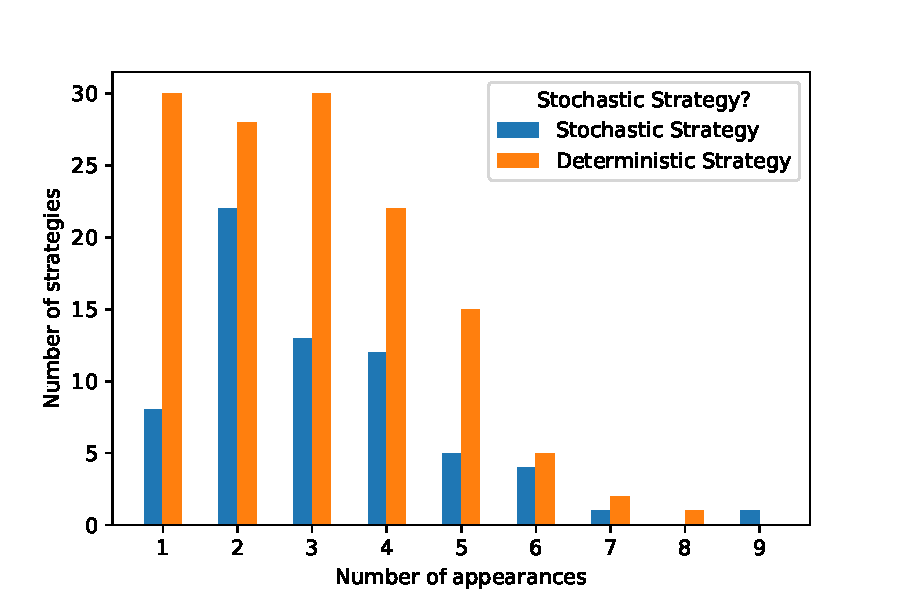
\includegraphics[width=\textwidth]{folk_thm/initial_analysis/strategy_appearances.pdf}
    \caption{A plot to show the ratio of stochastic to deterministic strategies randomly chosen throughout the experiment.}\label{fig:stochastic_chart}
\end{figure}

It is clear that there is a clear bias towards deterministic strategies
in this experiment. However, this is to be expected as running the following
code:
\begin{minted}[frame=lines, framesep=2mm, fontsize=\scriptsize, bgcolor=Cornsilk]{python}
    
    len(axl.filtered_strategies(filterset={"stochastic": True})), 
    len(axl.filtered_strategies(filterset={"stochastic": False}))

    (86, 156)
\end{minted}
it can be seen that over half the strategies coded into the Axelrod library are
classed as deterministic. Looking at Figure~\ref{fig:stochastic_chart} again,
observe, the majority of deterministic strategies were executed either once or
three times. On the other hand, a large proportion of the stochastic strategies
were played twice.

Further, the number of Nash equilibria obtained for each game was analysed and
their distributions with respect to the number of opponents of the
\textit{Defector} plotted. Executing the \textit{value\_counts} method on the
`num\_of\_equilibria' column gave the conclusion that the majority of games
(131773) yielded one Nash equilibria with 28793 games obtaining 3 equilibria.
Also, the maximum number of equilibria yielded, 39, was for one game, which,
doing a search on the database, was found to be a six player game with
noise=0.1. The opponents of the \textit{Defector} were: \textit{Inverse
Punisher}; \textit{Prober}; \textit{PSO Gambler 2\_2\_2 Noise 05};
\textit{Handshake}; and \textit{More Tideman and Chieruzzi}.

Figure~\ref{fig:NE_violinplot} shows the distributions of the number of Nash
equilibria as per the number of players. Observe, all of the distributions
observed on this plot have a clear modal value of one, that is, irrespective of
the number of players, the majority of games yielded only one equilibria. As can
be seen from the plot, the variance in the number of equilibria increases with
the number of players, apart from when there were 6 players (5 opponents of the
defector), where the spread is maximum. This could be due to the 39 equilibria
gained for one game as discussed in the paragraph above. Looking now at the mean
of the distributions, observe that these are also slightly increasing as the
number of players increase. 

\begin{figure}      
    \centering
    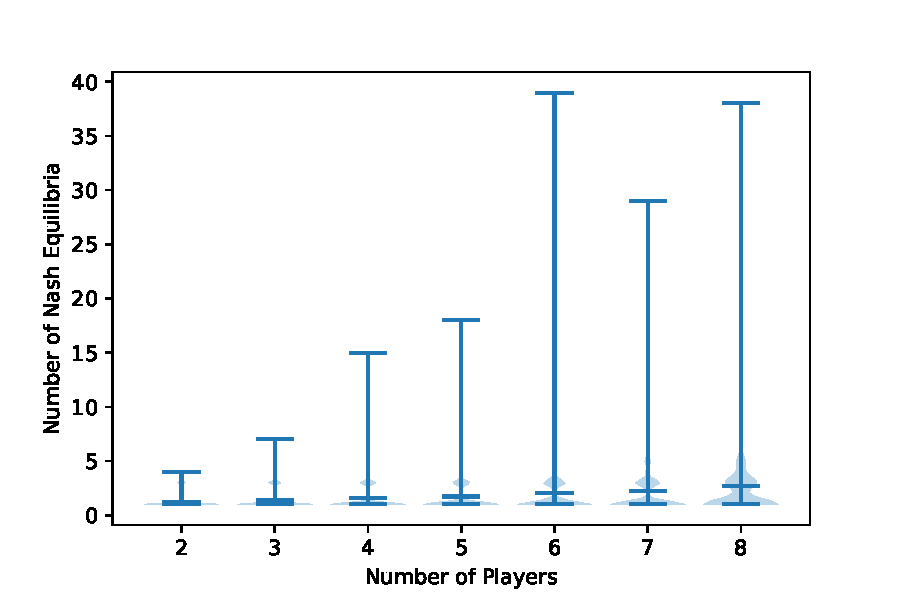
\includegraphics[width=\textwidth]{folk_thm/initial_analysis/player_num_of_equilibria_violinplot.pdf}
    \caption{A violinplot showing the distribution of the number of equilibria obtained for varying number of players.}\label{fig:NE_violinplot}
\end{figure}



\section{Analysis of the p-Threshold}\label{sec:Analysis_of_the_p-Threshold}
In order to analyse the \(p\)-thresholds of the tournaments, two csv files were
created~\footnote{Please see Appendix~\ref{} %TODO
for the code used to obtain these files.} containing the
minimum, mean, median and maximum probabilities for each set of tournaments.
This was in order to gain as much information as possible from tournaments which
gave graphs as shown in Figure~\ref{fig:less_clear}. That is, tournaments in
which the number of repetitions was not sufficient to omit the `noise' which
could affect the results.

\begin{figure}
    \begin{subfigure}{.3\textwidth}
        \centering
        \includegraphics[width=\textwidth]{folk_thm/single_game/8/157/0.0/main.pdf}
        \caption{This was an eight player tournament with no added noise. The opponent strategies were: \textit{Tester}; \textit{Gradual Killer: (D, D, D, D, D, C, C)}; \textit{Win-Shift Lose-Stay: D}; \textit{Evolved FSM 16}; \textit{Limited Retaliate: 0.1, 20}; \textit{ZD-GEN-2: 0.125, 0.5, 3}; and \textit{Joss: 0.9}.}
    \end{subfigure}
    \begin{subfigure}{.3\textwidth}
        \centering
        \includegraphics[width=\textwidth]{folk_thm/single_game/5/80/0.0/main.pdf}
        \caption{This was a five player tournament with no added noise. The opponent strategies were: \textit{WmAdams}; \textit{Joss: 0.9}; \textit{Yamachi}; and \textit{Stochastic WSLS:\@ 0.05}.}
    \end{subfigure}
    \begin{subfigure}{.3\textwidth}
        \centering
        \includegraphics[width=\textwidth]{folk_thm/single_game/2/24/0.0/main.pdf}
        \caption{This was a two player tournament with no added noise. The \textit{Defector}'s opponent was \textit{Fortress3}.}
    \end{subfigure}
    \caption{Examples of plots where the \(p\)-threshold isn't as clear.}\label{fig:less_clear}
\end{figure}

For clarity, here is a restatement of the definition of a
\textit{\(p\)-threshold}: The probability of the tournament ending for which the
least probability of defection in Nash equilibria is non-zero.

The first csv file created ignored whether a game could be degenerate and, by a
small alteration, the second file contained only the non-degenerate games. This
was in order to help identify whether degeneracy has any effect on the
\(p\)-threshold. Within these files, other than the varying thresholds, the
information about the number of players, tournament strategy set and level of
noise was retained.

Firstly, an exploration into the overall \(p\)-thresholds is given.

\begin{figure}
    \begin{subfigure}{.45\textwidth}
        \centering
        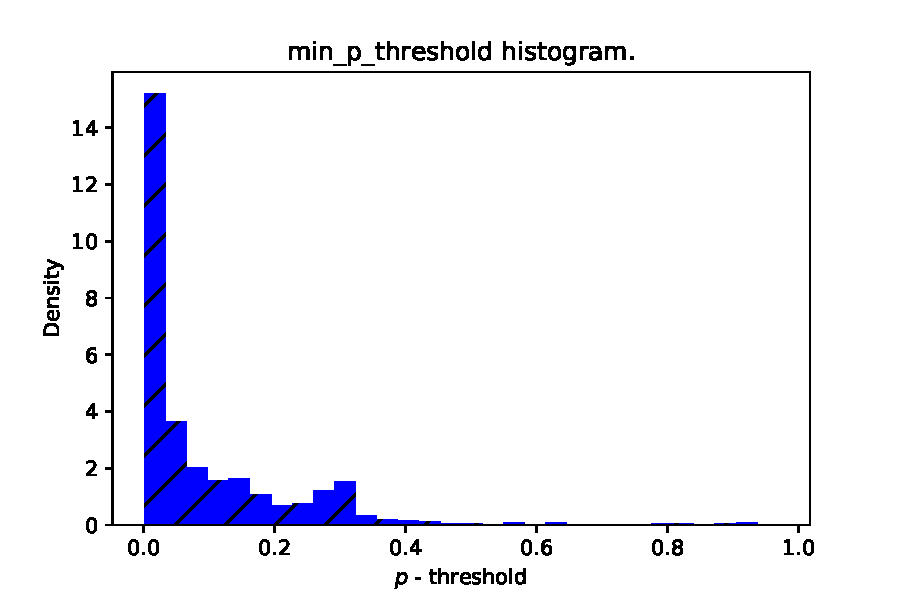
\includegraphics[width=\textwidth]{folk_thm/main_analysis/min_p_threshold_hist.pdf}
        \caption{A plot to show the minimum \(p\)-thresholds.}\label{subfig:min_p_thresh}
    \end{subfigure}
    \begin{subfigure}{.45\textwidth}
        \centering
        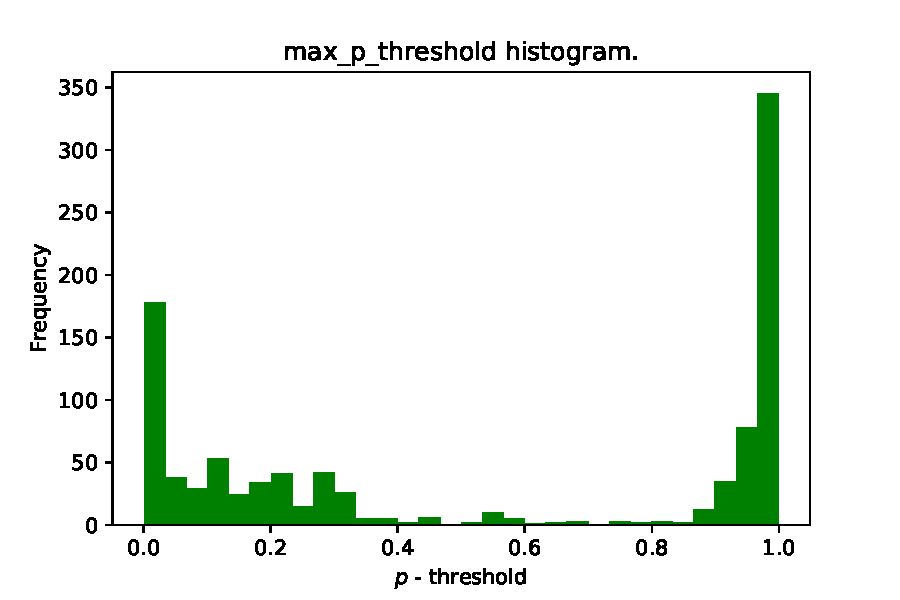
\includegraphics[width=\textwidth]{folk_thm/main_analysis/max_p_threshold_hist.pdf}
        \caption{A plot to show the maximum \(p\)-thresholds.}\label{subfig:max_p_thresh}
    \end{subfigure}
    \caption{Plots to show the \(p\)-thresholds for all 1001 sets of tournaments.}\label{fig:min_max_p_thresh}
\end{figure}

Observe, in Figure~\ref{subfig:min_p_thresh}, the majority of minimum thresholds
were less than 0.4, with a clear modal value of 0. That is, in a significant
proportion of the tournaments, there was no probability of the game ending for
which the probability of defection was zero. Now considering
Figure~\ref{subfig:max_p_thresh}, it can be seen that the modal value for the
maximum threshold is 1.
Also, in comparison with the minimum threshold, there is a larger spread in the
density. Yet, there is still a peak around zero as with the minimum threshold
data. Looking at the mean and median threshold data,
Figure~\ref{fig:mean_median_p_thresh}, observe that the distributions obtained
are similar with, again, a modal value of zero, indicating there is always a
chance of defection irrespective of the game ending probability. However, in
these histograms there is also a clear peak around a threshold of 0.5. This
suggests that some of the tournaments may have several p-thresholds, perhaps due
to stochasticity or degeneracy. Indeed, obtaining the minimum and maximum
p-thresholds for those tournaments where the mean threshold was within the range
\([0.5, 0.6]\), it can be seen that, from Figure~\ref{fig:p_mean_middle_plot}for a significant proportion, their minimum
threshold was around zero and their maximum around one. Moreover, looking closer
at three of the tournaments which satisfied the above, there is a clear
stochasticity within the corresponding graphs, Figure~\ref{fig:p_mean_middle_specific}.

\begin{figure}
    \begin{subfigure}{.45\textwidth}
        \centering
        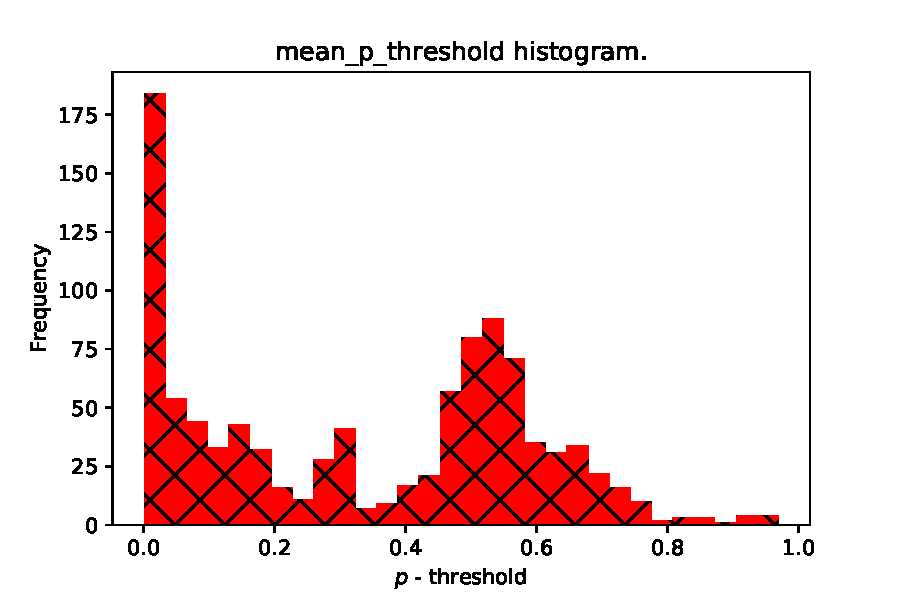
\includegraphics[width=\textwidth]{folk_thm/main_analysis/mean_p_threshold_hist.pdf}
        \caption{A plot to show the mean \(p\)-thresholds.}\label{subfig:mean_p_thresh}
    \end{subfigure}
    \begin{subfigure}{.45\textwidth}
        \centering
        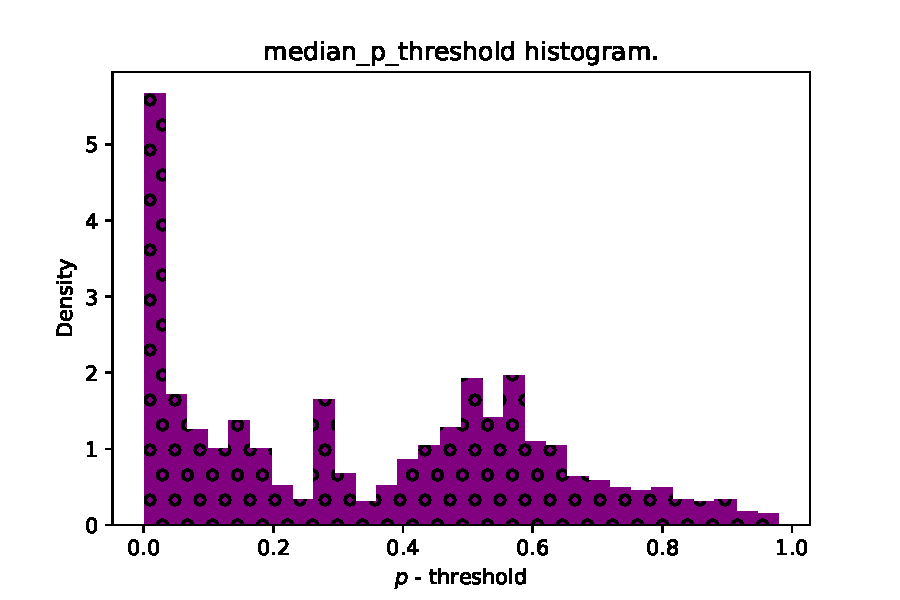
\includegraphics[width=\textwidth]{folk_thm/main_analysis/median_p_threshold_hist.pdf}
        \caption{A plot to show the median \(p\)-thresholds.}\label{subfig:median_p_thresh}
    \end{subfigure}
    \caption{Plots to show the \(p\)-thresholds for all 1001 sets of tournaments.}\label{fig:mean_median_p_thresh}
\end{figure}


\begin{figure}
    \centering
    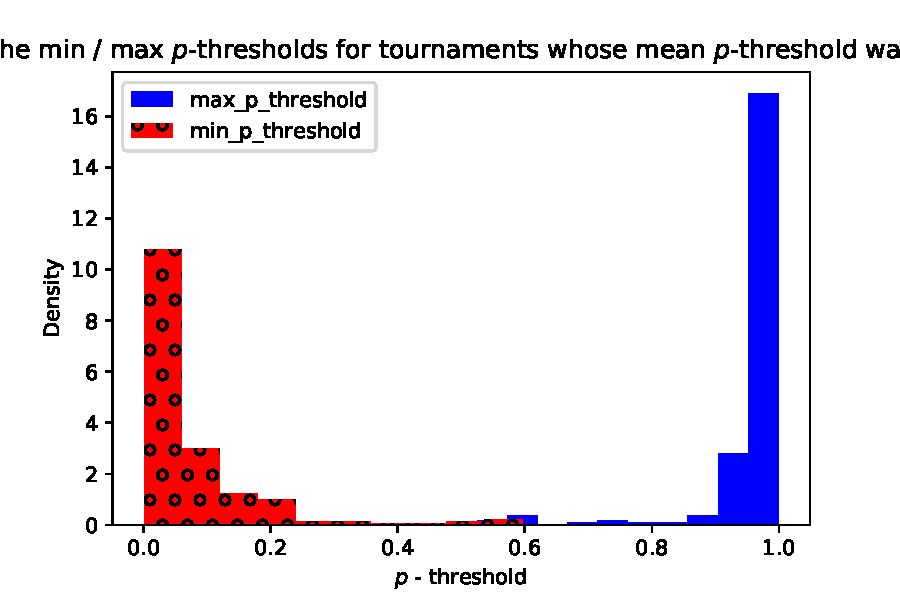
\includegraphics[width=\textwidth]{folk_thm/main_analysis/p_mean_middle_data_plot.pdf}
    \caption{A plot to show the minimum and maximum \(p\)-thresholds for those tournaments which had an mean threshold within the range \([0.5, 0.6]\).}\label{fig:p_mean_middle_plot}
\end{figure}


\begin{figure}
    \begin{subfigure}{0.3\textwidth}
        \centering
        \includegraphics[width=\textwidth]{folk_thm/single_game/6/105/0.2/main.pdf}
        \caption{This plot was obtained from the tournament in which the five
        opponents of the \textit{Defector} were: \textit{RichardHufford};
        \textit{Soft Joss: 0.9}; \textit{Feld: 1.0, 0.5, 200};
        \textit{UsuallyDefects}; and \textit{Handshake}. The tournament also included an additional 0.2 of noise.}
    \end{subfigure}
    \begin{subfigure}{0.3\textwidth}
        \centering
        \includegraphics[width=\textwidth]{folk_thm/single_game/3/35/0.1/main.pdf}
        \caption{This plot represents the, 0.1 noise, tournament with the three players: \textit{Worse and Worse 2}; \textit{Raider}; and, \textit{Defector}.}
    \end{subfigure}
    \begin{subfigure}{0.3\textwidth}
        \centering
        \includegraphics[width=\textwidth]{folk_thm/single_game/3/33/0.5/main.pdf}
        \caption{This plot was produced from the tournament in which the \textit{Defector} was playing \textit{ZD-Extort-2: 0.1111111111111111, 0.5} and \textit{Adaptive Tit For Tat: 0.5}. There was the addition of 0.5 noise within the tournament.}
    \end{subfigure}
    \caption{Example plots of the tournaments where the mean \(p\)-threshold was within the range \([0.5, 0.6]\).}\label{fig:mean_middle_specific}
\end{figure}

Before continuing onto the general overview of the thresholds for those
tournaments which led to definite non-degenerate games, a brief point is made
regarding those tournaments which, for all probabilities of the game ending, had
no positive probability of defection. Indeed, out of the 1754 total tournaments
753 of them had the above property of no threshold. That is, the plots obtained
for these tournaments were (approximately) constant at zero for all
probabilities of the game ending. Further investigation into these tournaments
will be executed later. 

Regarding degeneracy, out of all 1754 tournaments, 372 were highlighted as
potentially leading to degenerate games. Furthermore, out of those tournaments
which had a p-threshold, 253 of them were identified as possibly degenerate.
These are omitted from the following plots in order to focus solely on
non-degenerate games.

\begin{figure}
    \begin{subfigure}{.45\textwidth}
        \centering
        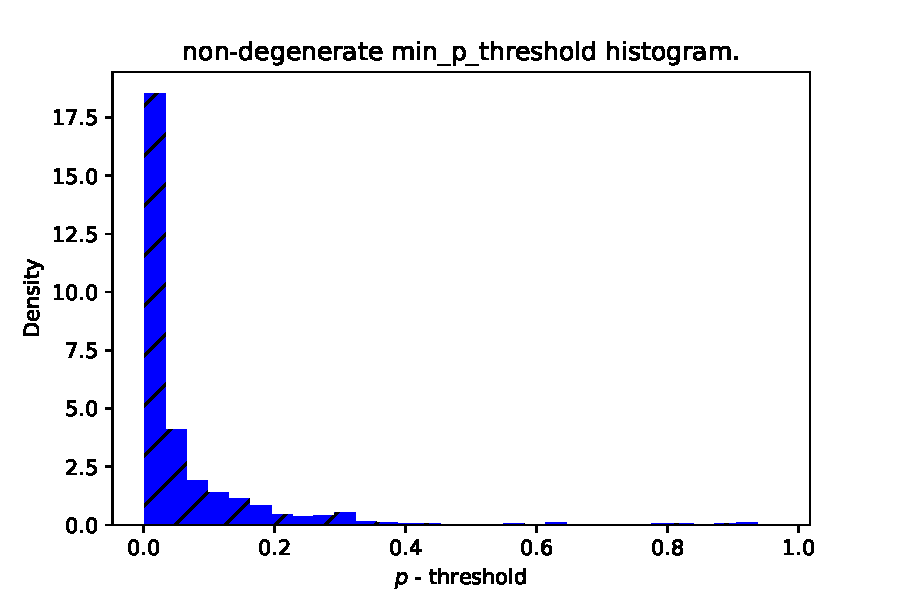
\includegraphics[width=\textwidth]{folk_thm/main_analysis/non-degen_min_p_threshold_hist.pdf}
        \caption{A plot to show the minimum \(p\)-thresholds.}\label{subfig:non_degen_min_p_thresh}
    \end{subfigure}
    \begin{subfigure}{.45\textwidth}
        \centering
        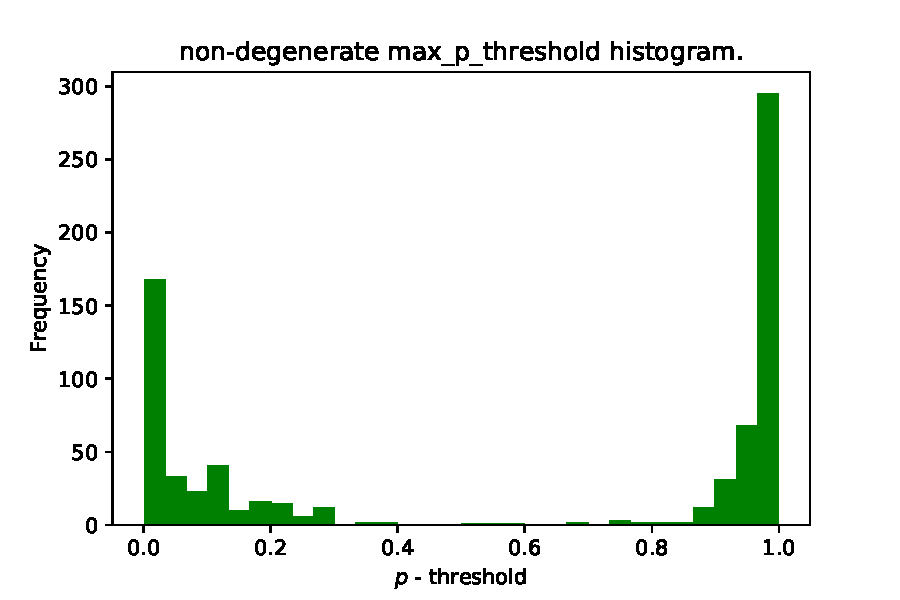
\includegraphics[width=\textwidth]{folk_thm/main_analysis/non-degen_max_p_threshold_hist.pdf}
        \caption{A plot to show the maximum \(p\)-thresholds.}\label{subfig:non_degen_max_p_thresh}
    \end{subfigure}
    \caption{Plots to show the \(p\)-thresholds for all tournaments which led to non-degenerate games.}\label{fig:non_degen_min_max_p_thresh}
\end{figure}


\begin{figure}
    \begin{subfigure}{.45\textwidth}
        \centering
        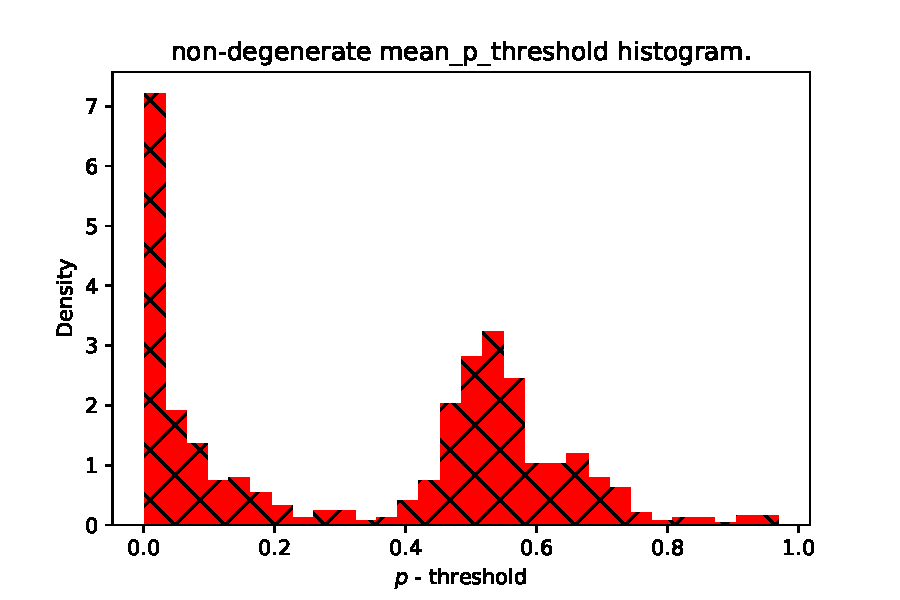
\includegraphics[width=\textwidth]{folk_thm/main_analysis/non-degen_mean_p_threshold_hist.pdf}
        \caption{A plot to show the mean \(p\)-thresholds.}\label{subfig:non_degen_mean_p_thresh}
    \end{subfigure}
    \begin{subfigure}{.45\textwidth}
        \centering
        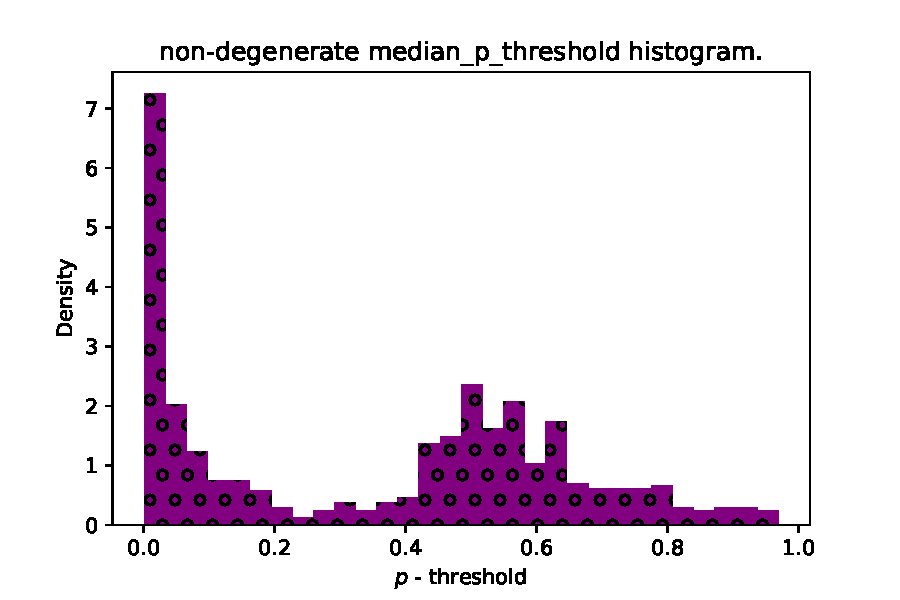
\includegraphics[width=\textwidth]{folk_thm/main_analysis/non-degen_median_p_threshold_hist.pdf}
        \caption{A plot to show the median \(p\)-thresholds.}\label{subfig:non_degen_median_p_thresh}
    \end{subfigure}
    \caption{Plots to show the \(p\)-thresholds for all tournaments which led to non-degenerate games.}\label{fig:non_degen_mean_median_p_thresh}
\end{figure}

Comparing Figures~\ref{subfig:non_degen_min_p_thresh},~\ref{subfig:non_degen_max_p_thresh},~\ref{subfig:non_degen_mean_p_thresh}
and~\ref{subfig:non_degen_median_p_thresh} with 
Figures~\ref{subfig:min_p_thresh},~\ref{subfig:max_p_thresh},~\ref{subfig:mean_p_thresh}
and~\ref{subfig:median_p_thresh}, respectively, it can be seen that, in general,
there is no significant change in the distributions of the thresholds. However,
there is a more prominent peak in Figure~\ref{subfig:mean_p_thresh} around 0.3
than in the corresponding non-degenerate plot of
Figure~\ref{subfig:non_degen_mean_p_thresh}. The effects of degeneracy will be
investigated in more depth in Section~\ref{subsec:Effects_of_Degeneracy}. 


\subsection{Effects of the Number of Players}\label{subsec:Effects_of_the_number_of_Players}
In this section, the \(p\)-thresholds will be analysed with respect to the
number of opponents the \textit{Defector} played against. Note, in this section,
only non-degenerate tournaments will be considered.


\begin{figure}
    \centering
    \begin{subfigure}{0.45\textwidth}
        \centering
        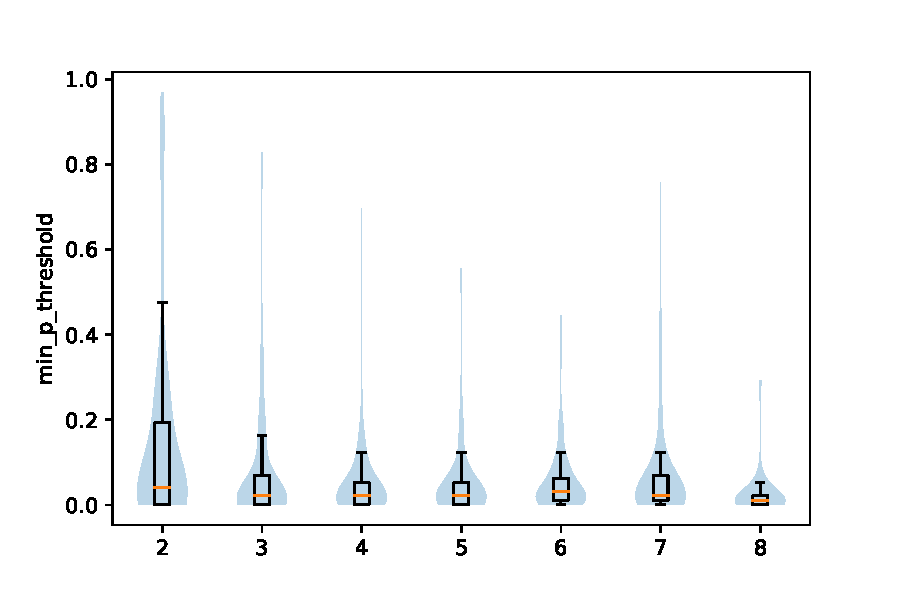
\includegraphics[width=\textwidth]{folk_thm/main_analysis/min_p_threshold_player_violinplot.pdf}
        \caption{Minimum p-threshold violinplot.}\label{subfig:min_thresh_player_violinplot}
    \end{subfigure}
    \begin{subfigure}{0.45\textwidth}
        \centering
        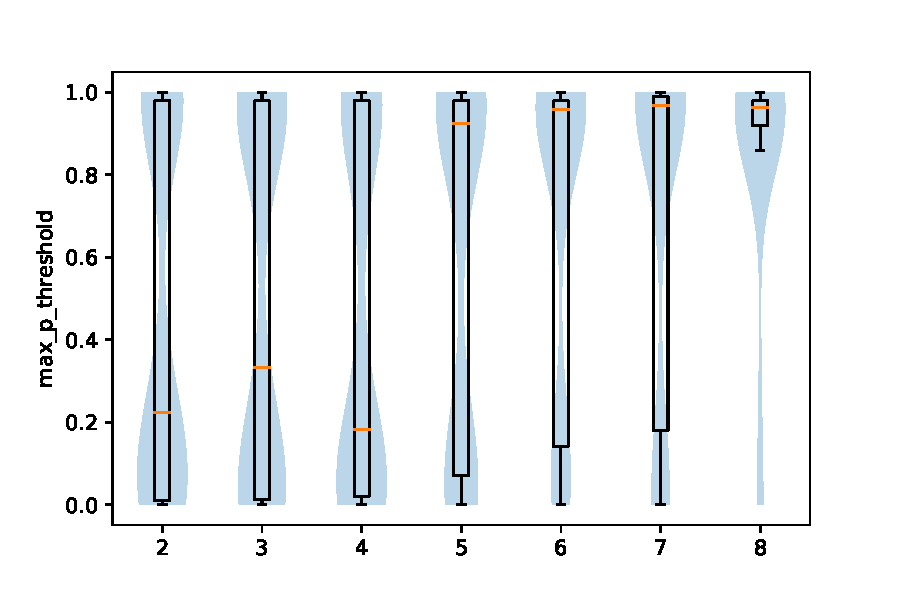
\includegraphics[width=\textwidth]{folk_thm/main_analysis/max_p_threshold_player_violinplot.pdf}
        \caption{Maximum p-threshold violinplot.}\label{subfig:max_thresh_player_violinplot}
    \end{subfigure}

    \begin{subfigure}{0.45\textwidth}
        \centering
        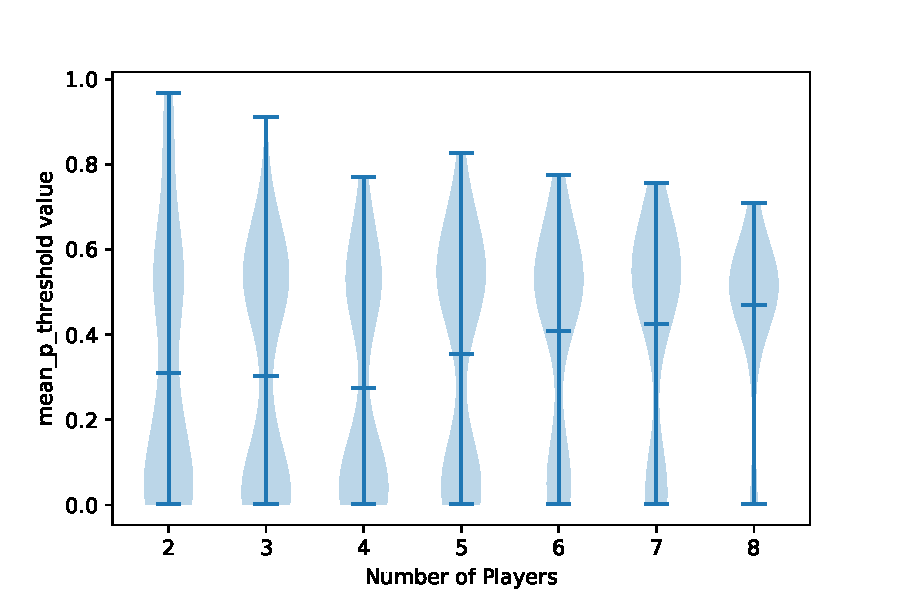
\includegraphics[width=\textwidth]{folk_thm/main_analysis/mean_p_threshold_player_violinplot.pdf}
        \caption{Mean p-threshold violinplot.}\label{subfig:mean_thresh_player_violinplot}        
    \end{subfigure}
    \begin{subfigure}{0.45\textwidth}
        \centering
        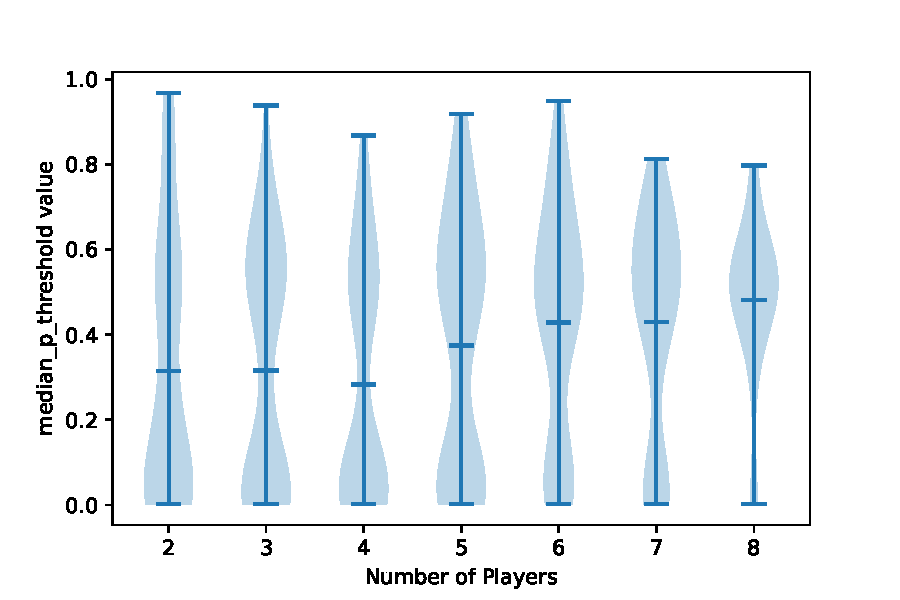
\includegraphics[width=\textwidth]{folk_thm/main_analysis/median_p_threshold_player_violinplot.pdf}
        \caption{Median p-threshold violinplot.}\label{subfig:median_thresh_player_violinplot}
    \end{subfigure}
    \caption{Violinplots of the thresholds for each number of opponents.}\label{fig:player_mean_thresh_violinplot}
\end{figure}

From Figure~\ref{subfig:mean_thresh_player_violinplot}, it can be seen that the
distributions of the minimum \(p\)-thresholds with respect to the number of
players all have a modal value around 0. However, apart from the 7-player
tournaments, the spread of the distributions decrease, along with the mean
values. Considering the maximum thresholds,
Figure~\ref{subfig:max_p_threshold_violinplot}, the distributions become bimodal
with mode values of around 0 and 1. But, as the number of players increases the
modal value at zero becomes less prominent with the 8-player tournament
distribution not having a mode around 0. The variance of the distributions are
similar and, apart from 4-player tournaments, the means increase with the number
of players. Looking now to the mean and median violinplots,
Figures~\ref{subfig:mean_thresh_player_violinplot}
and~\ref{subfig:median_thresh_player_violinplot} respectively, there is no
significant difference between the two plots other than the spread is a little
larger in the median thresholds. Within the mean plot,
Figure~\ref{subfig:mean_thresh_player_violinplot}, it can be seen that the
distributions also start off bimodal, at 0 and approximately 0.5. But again, the
modal value at zero becomes less distinct with the 8-player tournament
distribution being unimodal. The modal value at around 0.5 is a consequence of
the reason stated in the previous section. Moreover, observe that, apart from
4-player tournaments, the variance of the distributions seem to decrease with
the size of the player set whilst the means increase from a value of
approximately 0.3 for 2-player tournaments to around 0.5 for 8-players.


\subsection{Effects of Stochastic Players}\label{subsec:Effects_of_Stochastic_Players}

In order to analyse the effect of stochastic strategies on the \(p\)-threshold,
tournaments in which these strategies featured are repeated but any
stochastic players are omitted to identify any alterations in the results. 




\subsection{Effects of Noise}\label{subsec:Effects_of_Noise}

Here, an analysis on the effects of noise on the \(p\)-threshold is provided.
The addition of noise to a tournament indicates that, with a certain
probability, the action of a particular strategy is
altered~\cite{glynatsi2020meta}. That is, an action of \textit{coop} changes to
\textit{defect} and vice versa.  

\begin{figure}
    \begin{subfigure}{.45\textwidth}
        \centering
        \includegraphics[width=\textwidth]{{folk_thm/main_analysis/0.0noise_mean_p_thresh}.pdf}
        \caption{A plot to show the mean \(p\)-thresholds for all tournaments with no added noise.}\label{subfig:0.0noise_mean_p_thresh}
    \end{subfigure}
    \begin{subfigure}{.45\textwidth}
        \centering
        \includegraphics[width=\textwidth]{{folk_thm/main_analysis/0.1noise_mean_p_thresh}.pdf}
        \caption{A plot to show the mean \(p\)-thresholds for all tournaments with noise = 0.1.}\label{subfig:0.1noise_mean_p_thresh}
    \end{subfigure}

    \begin{subfigure}{.3\textwidth}
        \centering
        \includegraphics[width=\textwidth]{{folk_thm/main_analysis/0.2noise_mean_p_thresh}.pdf}
        \caption{A plot to show the mean \(p\)-thresholds for all tournaments with noise = 0.2.}\label{subfig:0.2noise_mean_p_thresh}
    \end{subfigure}
    \begin{subfigure}{.3\textwidth}
        \centering
        \includegraphics[width=\textwidth]{{folk_thm/main_analysis/0.3noise_mean_p_thresh}.pdf}
        \caption{A plot to show the mean \(p\)-thresholds for all tournaments with noise = 0.3.}\label{subfig:0.3noise_mean_p_thresh}
    \end{subfigure}
    \begin{subfigure}{.3\textwidth}
        \centering
        \includegraphics[width=\textwidth]{{folk_thm/main_analysis/0.4noise_mean_p_thresh}.pdf}
        \caption{A plot to show the mean \(p\)-thresholds for all tournaments with noise = 0.4.}\label{subfig:0.4noise_mean_p_thresh}
    \end{subfigure}

    \begin{subfigure}{.3\textwidth}
        \centering
        \includegraphics[width=\textwidth]{{folk_thm/main_analysis/0.5noise_mean_p_thresh}.pdf}
        \caption{A plot to show the mean \(p\)-thresholds for all tournaments with noise = 0.5.}\label{subfig:0.5noise_mean_p_thresh}
    \end{subfigure}
    \begin{subfigure}{.3\textwidth}
        \centering
        \includegraphics[width=\textwidth]{{folk_thm/main_analysis/0.6noise_mean_p_thresh}.pdf}
        \caption{A plot to show the mean \(p\)-thresholds for all tournaments with noise = 0.6.}\label{subfig:0.6noise_mean_p_thresh}
    \end{subfigure}
    \begin{subfigure}{.3\textwidth}
        \centering
        \includegraphics[width=\textwidth]{{folk_thm/main_analysis/0.7noise_mean_p_thresh}.pdf}
        \caption{A plot to show the mean \(p\)-thresholds for all tournaments with noise = 0.7.}\label{subfig:0.7noise_mean_p_thresh}
    \end{subfigure}
    \begin{subfigure}{.3\textwidth}
        \centering
        \includegraphics[width=\textwidth]{{folk_thm/main_analysis/0.8noise_mean_p_thresh}.pdf}
        \caption{A plot to show the mean \(p\)-thresholds for all tournaments with noise = 0.8.}\label{subfig:0.8noise_mean_p_thresh}
    \end{subfigure}
    \begin{subfigure}{.3\textwidth}
        \centering
        \includegraphics[width=\textwidth]{{folk_thm/main_analysis/0.9noise_mean_p_thresh}.pdf}
        \caption{A plot to show the mean \(p\)-thresholds for all tournaments with noise = 0.9.}\label{subfig:0.9noise_mean_p_thresh}
    \end{subfigure}
    \begin{subfigure}{.3\textwidth}
        \centering
        \includegraphics[width=\textwidth]{{folk_thm/main_analysis/1.0noise_mean_p_thresh}.pdf}
        \caption{A plot to show the mean \(p\)-thresholds for all tournaments with noise = 1.0.}\label{subfig:1.0noise_mean_p_thresh}
    \end{subfigure}
    \caption{Plots to show the mean \(p\)-threshold for varying levels of noise.}\label{fig:noise_mean_p_thresh}
\end{figure}


Figure~\ref{fig:noise_mean_p_thresh} shows the mean \(p\)-thresholds for all
non-degenerate tournaments with the addition of varying probabilities of noise.
Firstly, observe that for those tournaments with the addition of noise at least
0.6
(Figures~\ref{subfig:0.6noise_mean_p_thresh},~\ref{subfig:0.6noise_mean_p_thresh},~\ref{subfig:0.6noise_mean_p_thresh},~\ref{subfig:0.6noise_mean_p_thresh},~\ref{subfig:0.6noise_mean_p_thresh})
the majority of thresholds are equal to one. This is due to the definition of
the parameter noise in the tournaments as described above, That is, there is a
greater chance that the \textit{Defector's} strategy will change to cooperation.
Hence, only tournaments with noise\(\le 0.5\) will be considered. 


\begin{figure}
    \centering
    \includegraphics[width=\textwidth]{folk_thm/main_analysis/noise_mean_thresh_violinplot.pdf}
    \caption{A violinplot showing the distribution of mean \(p\)-thresholds for each level of noise.}\label{fig:noise_mean_thresh_violinplot}
\end{figure}



\subsection{Effects of Degeneracy}\label{subsec:Effects_of_Degeneracy}

\section{Multivariate Data Analysis}\label{sec:MV_Data_Analysis}

\section{Reliability of Data}\label{sec:Reliability_of_Data}

\subsection{Comparison of Databases}\label{subsec:Comparison_of_Databases}

\subsection{Accuracy of Thresholds}\label{subsec:Accuracy_of_Thresholds}